\documentclass[11pt,a4paper]{article}
\usepackage[margin=21mm]{geometry}
\usepackage[T1]{fontenc}
\usepackage{lmodern,booktabs,graphicx,amsmath,hyperref,float}
\hypersetup{hypertexnames=false,colorlinks=true,urlcolor=blue,linkcolor=blue,pdftitle={Permutation inference for displaced/non-displaced EEG decoding},pdfauthor={Satyam Awasthi}}
\setlength{\emergencystretch}{2em}
\setlength{\parindent}{0pt}\setlength{\parskip}{5pt}
\title{Permutation inference for displaced/non-displaced EEG decoding}
\author{Satyam Awasthi}\date{}
\begin{document}\maketitle
\section{Question and fixed primary analysis}
Does the fixed eight-channel, 100 ms shrinkage-LDA decoder exceed a participant-specific label-shuffled chance distribution under the existing whole-recording validation? The 23 non-pilot participants form the primary evaluation. mle01 and spe30 informed feature/model selection and remain explicitly exploratory. This note complements the earlier classification results and the participant/session waveform figures.

The primary pipeline is continuous 1--20 Hz BP no-FORCe, with the same accepted trial IDs, event alignment, baseline and quality checks as the saved decoder analysis. Seven 100 ms means per channel over $[0.2,0.9)$ s provide 56 features. Standardisation and shrinkage LDA (equal class priors, automatic covariance shrinkage) are fitted on training recordings only. No preprocessing or model tuning is repeated or changed here.

\section{Permutation method and statistic}
We draw 1,999 random label permutations independently within each recording, preserving its D/ND counts. Each permutation refits the models using exactly the existing leave-one-recording-out folds, separately within participant/session. Test predictions are pooled within a session before computing balanced accuracy (mean D/ND recall). Participant statistics average eligible session scores equally; each participant's null statistic uses the same aggregation. Exclusions remain rle13/pre and vco27/pre, whose training folds cannot support the protocol. The analysis covers 73 eligible sessions and 30,210 evaluated trials.

The one-sided Monte Carlo value is
\[
p=\frac{1+\#\{b:T_b\ge T_{\mathrm{obs}}\}}{1+1999},
\]
with ties included and minimum attainable $p=0.0005$. Chance$_{95}$ is the empirical 95th percentile of the null (upper order statistic), an unadjusted descriptive threshold. Holm adjustment controls family-wise error across the 23 primary participant tests. Session-level values in the web report are unadjusted exploratory checks, not additional corrected primary claims.

The web report also includes central LDA, the all-eight-channel binned tree, and the Graz-style top-100 amplitude tree. The latter reranks all 8,000 full-epoch candidates using training data inside every permutation and fold. These 69 secondary non-pilot tests form a separate Holm family. The eight pilot/model tests form an exploratory family; correction does not remove bias from earlier pilot model/feature selection. Observed held-out predictions for all four models are checked against the saved analyses.

\clearpage
\section{Primary participant results}
Eight-channel shrinkage LDA exceeded the within-recording label-shuffle null after Holm correction in 23/23 non-pilot participants. The unadjusted participant-specific 95th-percentile chance thresholds ranged from 52.6\% to 54.9\%. The Holm-corrected $p$-values determine significance after adjustment.
Raw primary p-values ranged from 0.0005 to 0.0065. The Monte Carlo minimum of 0.0005 occurred for 22/23 participants. All primary Holm-adjusted p-values were 0.0115.

\begin{table}[H]\centering\small\setlength{\tabcolsep}{4pt}
\begin{tabular}{@{}lrrrrrr@{}}\toprule
Participant & Sessions & Trials & BA (\%) & Chance$_{95}$ (\%) & $p$ & $p_{\mathrm{Holm}}$\\\midrule
ara13 & 3 & 1,325 & 84.2 & 53.1 & 0.0005 & 0.0115\\
bal08 & 3 & 1,261 & 87.4 & 52.9 & 0.0005 & 0.0115\\
bpe06 & 3 & 1,140 & 70.3 & 53.2 & 0.0005 & 0.0115\\
bro19 & 3 & 816 & 79.2 & 54.8 & 0.0005 & 0.0115\\
cna07 & 3 & 994 & 84.8 & 53.5 & 0.0005 & 0.0115\\
cve01 & 3 & 1,405 & 86.6 & 52.8 & 0.0005 & 0.0115\\
den12 & 3 & 1,364 & 71.1 & 52.7 & 0.0005 & 0.0115\\
eab31 & 3 & 1,423 & 66.3 & 52.9 & 0.0005 & 0.0115\\
emo24 & 3 & 884 & 74.4 & 53.9 & 0.0005 & 0.0115\\
fbo09 & 3 & 1,332 & 82.3 & 53.0 & 0.0005 & 0.0115\\
gba12 & 3 & 1,414 & 82.6 & 53.0 & 0.0005 & 0.0115\\
gcr27 & 3 & 1,439 & 73.4 & 53.3 & 0.0005 & 0.0115\\
lbo12 & 3 & 1,265 & 71.0 & 53.1 & 0.0005 & 0.0115\\
ldu23 & 3 & 1,275 & 72.6 & 53.3 & 0.0005 & 0.0115\\
meb17 & 3 & 1,010 & 72.1 & 53.4 & 0.0005 & 0.0115\\
mka24 & 3 & 1,398 & 77.2 & 52.9 & 0.0005 & 0.0115\\
nfu22 & 3 & 1,435 & 80.8 & 52.6 & 0.0005 & 0.0115\\
nsh23 & 3 & 1,442 & 71.8 & 52.7 & 0.0005 & 0.0115\\
rle13 & 2 & 887 & 86.1 & 53.6 & 0.0005 & 0.0115\\
sga12 & 3 & 1,121 & 72.5 & 53.2 & 0.0005 & 0.0115\\
sto20 & 3 & 1,291 & 71.9 & 53.2 & 0.0005 & 0.0115\\
vco27 & 2 & 612 & 56.8 & 54.4 & 0.0065 & 0.0115\\
yle21 & 3 & 1,112 & 79.6 & 54.9 & 0.0005 & 0.0115\\
\bottomrule\end{tabular}

\caption{Non-pilot participants. BA is the equal-session mean balanced accuracy. Chance$_{95}$ uses the identical statistic under within-recording label permutations. Holm values refer to the 23-test primary family.}
\end{table}
\begin{table}[H]\centering\small\setlength{\tabcolsep}{4pt}
\begin{tabular}{@{}lrrrrrr@{}}\toprule
Participant & Sessions & Trials & BA (\%) & Chance$_{95}$ (\%) & $p$ & $p_{\mathrm{Holm}}$\\\midrule
mle01 & 3 & 1,179 & 75.9 & 53.0 & 0.0005 & 0.0040\\
spe30 & 3 & 1,386 & 85.8 & 52.7 & 0.0005 & 0.0040\\
\bottomrule\end{tabular}

\caption{Exploratory pilots, shown separately. Their Holm values belong to the eight-test pilot/model family; they are not independent validation of pilot-driven choices.}
\end{table}
The secondary model tables and unadjusted session checks are available in the existing DEC web report.

\clearpage
\section{Observed performance and chance thresholds}
\begin{figure}[H]\centering
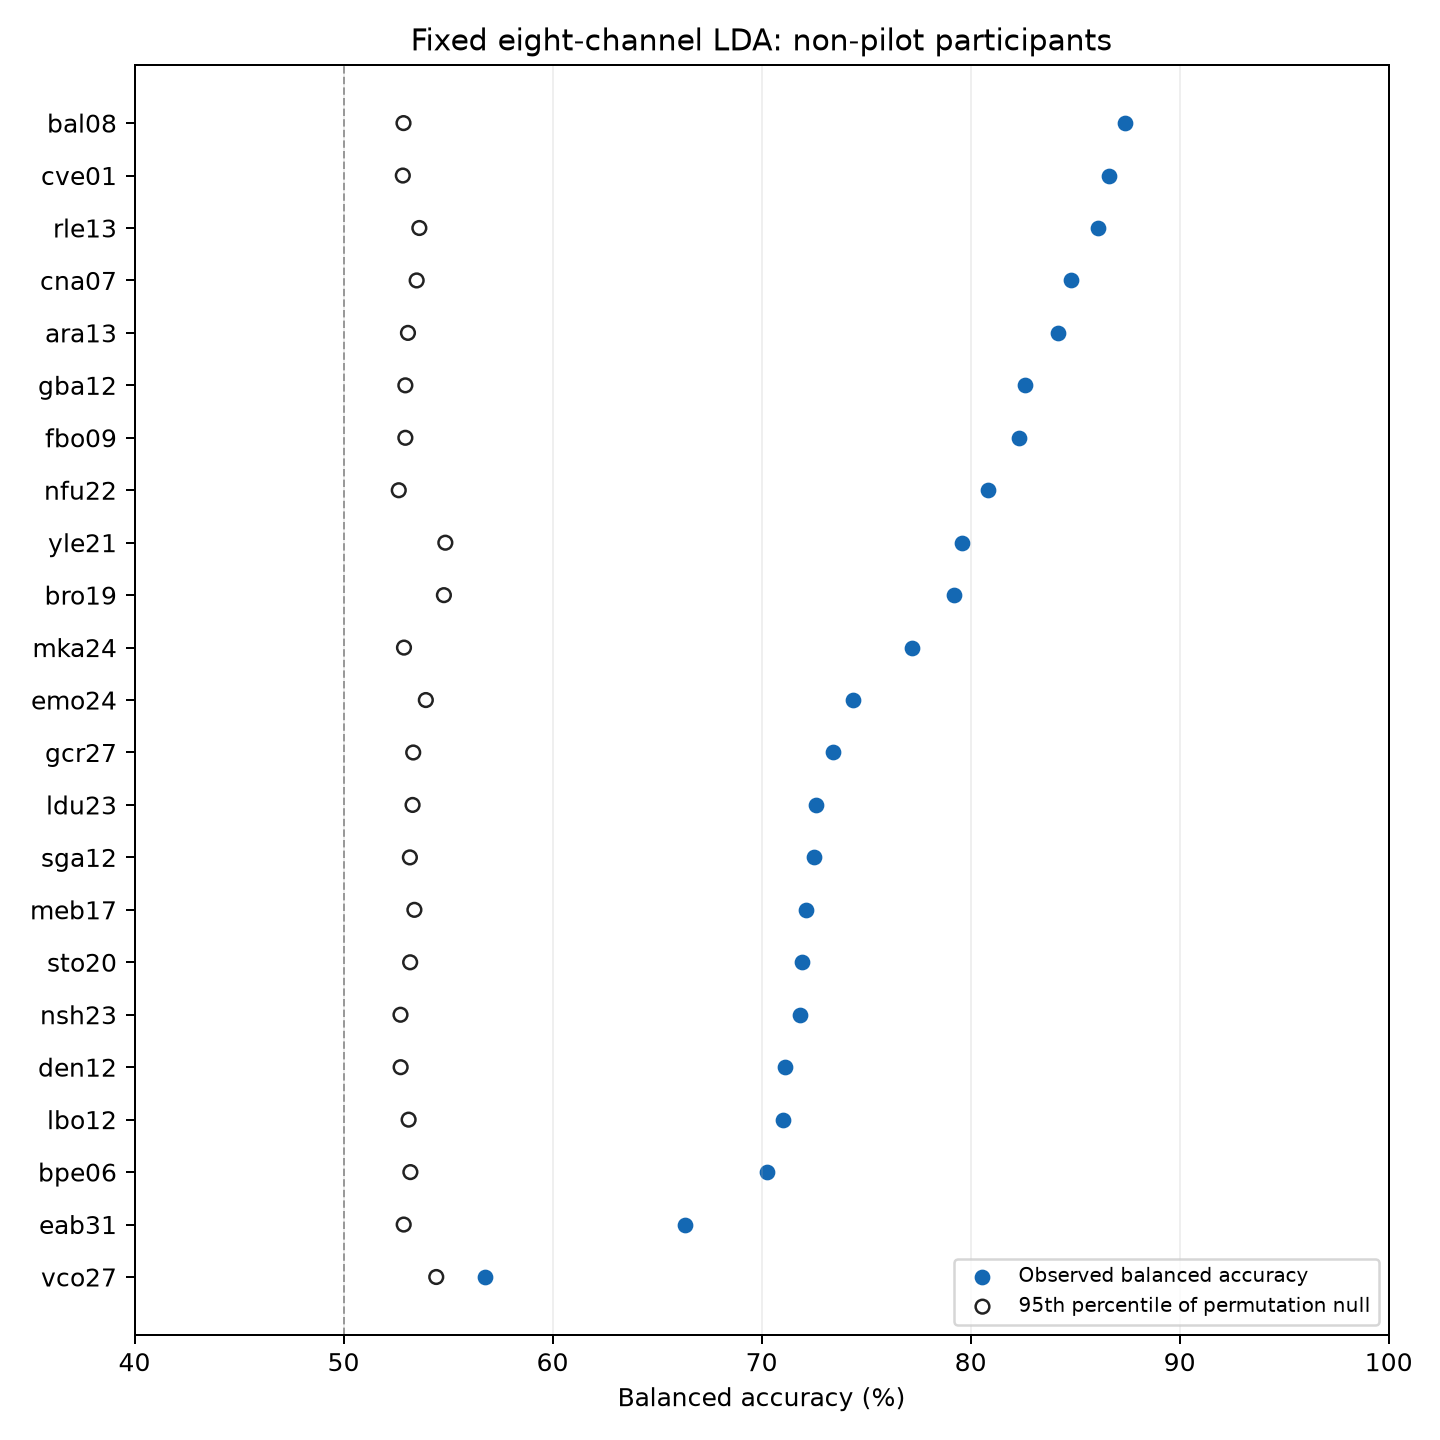
\includegraphics[width=.95\linewidth,height=.50\textheight,keepaspectratio]{figures/permutation_LDA_primary.png}
\caption{Observed participant scores and unadjusted permutation-derived thresholds for the primary LDA. The threshold markers are not confidence intervals or family-wise corrected decision thresholds.}
\end{figure}
\section{Interpretation and limits}
The null assumes D/ND labels are exchangeable within each recording. Blocking by recording preserves recording-level class proportions but does not establish exchangeability in the presence of unmodelled temporal structure. This is inference conditional on the existing trial inclusion and fixed personalised decoder, not a test of generalisation of a trained model to new participants.

Above-null discrimination supports useful label-related information. It does not identify an ErrP, establish error awareness, or rule out visual, movement-related or residual artifact contributions. Waveform morphology, timing and scalp distribution remain complementary evidence.

\small\textbf{Method references.} Ojala and Garriga, \emph{Permutation tests for studying classifier performance}, JMLR 11 (2010), 1833--1863. Phipson and Smyth, \emph{Permutation p-values should never be zero}, SAGMB 9 (2010), Article 39, doi:10.2202/1544-6115.1585. The implementation follows the grouped-shuffle and $+1$ Monte Carlo convention documented by scikit-learn.
\end{document}
